\chapter*{Introduzione}
\addcontentsline{toc}{chapter}{Introduzione}
Nell’era moderna la crescente quantità di dati di cui usufruiamo ogni giorno sta ricevendo, dagli esperti del settore, molte attenzioni. In quanto il troughput e la quantità di memoria di cui disponiamo sui nostri dispositivi sono, seppur ad oggi ampiamente sufficienti, comunque limitate. Un’altra ragione di questa attenzione è la crescente diffusione di servizi in tempo reale che quindi richiedono di scambiare quantità di dati considerevoli in pochissimo tempo. Un esempio di tali servizi potrebbe essere l’uso della realtà aumentata in ambito medico o di ricerca. Comprimere i dati è quindi ormai una necessità, che si farà sempre più impellente con il crescere delle dimensioni dei dati che andremo a gestire.
A partire dai primi anni primi anni novanta infatti si sono iniziate a sviluppare alcune tecniche, a cui oggi si fa rifermento come tecniche tradizionali, per comprimere le immagini. Stiamo parlando ed esempio di JPEG e del suo successore JPEG2000, di più recente sviluppo sono invece i codec BPG e VVC.
Più recentemente l’attenzione dei ricercatori si è spostata su metodi basati su deep learning. Questi metodi presentano diversi vantaggi rispetto ai metodi tradizionali, infatti molte volte permettono di ottenere performance migliori rispetto ai metodi classici.\\
In questo documento ci proponiamo di fornire una panoramica dei metodi di compressione tradizionali più usati, e di quelli basati su deep learning che hanno fornito un maggiore contributo allo sviluppo di questi ultimi. Dopo aver presentato le varie tecniche vogliamo fornirne una valutazione delle prestazioni, in modo da poterli comprare oggettivamente.\\
La compressione è un processo che mira a minimizzare il numero di bit utilizzati per rappresentare una certa informazione senza intaccarne drasticamente la qualità. Questo obbiettivo viene raggiunto riducendo le ridondanze e eliminando i dati irrilevanti.
Tutti i framework di compressione consistono di una coppia codificatore-decodificatore, in cui il codificatore ha il compito appunto di codificare l’immagine in una rappresentazione ridotta e il decodificatore trasforma la rappresentazione ridotta nuovamente in un’immagine.\\
Tutti gli algoritmi di compressione possono essere raggruppati in due macro categorie. Gli algoritmi lossy o con perdita e quelli lossless o senza perdita. Come si può già intuire dal nome gli algoritmi lossless comprimono le informazioni senza scartare informazioni, si limitano quindi ad applicare delle trasformate per ottenere delle nuove rappresentazioni più efficienti. Gli algoritmi lossy invece ammettono la possibilità di scartare delle informazioni superflue che non vanno ad intaccare drasticamente la qualità percepita dell’immagine, in modo da poter comprimere ulteriormente.
Se andiamo ad osservare gli algoritmi di codifica lossy possiamo scomporli tutti in almeno tre blocchi principali \cite{sadeeq2021image}, con l’aggiunta di un ulteriore blocco negli algoritmi più recenti, come possiamo vedere nel diagramma \ref{fig:LossyCompressorDiagram} \\
Un primo blocco si occupa di convertire l’immagine in una rappresentazione latente, tramite l’applicazione di una trasformata, in un altro dominio che permette di rappresentare l’informazione da comprimere in modo più sparso.\\
Successivamente si ha un blocco che si occupa di quantizzazione, ovvero di mappare i valori in ingresso in un insieme finito di dimensione più piccola rispetto a quello di ingresso. In questo passaggio si realizza la perdita di informazioni caratteristica della codifica lossy.\\
Un ultimo blocco si occupa di effettuare la codifica entropica, in modo da comprimere ulteriormente l’informazione mappando i simboli usati più spesso con pochi bit.\\
Il quarto blocco, che è stato aggiunto successivamente, si occupa di effettuare predizione spaziale, ovvero di sfruttare le ridondanze e le regioni omogenee delle immagini per comprimere ulteriormente, nonostante questo blocco sia stato introdotto per ultimo va a posizionarsi all’inizio, prima del blocco che applica la trasformata.
Data quindi un’immagine da comprimere $x$, il codificatore è composto sempre almeno da una trasformata  $\varepsilon$ e una funzione di quantizzazione $Q$. Negli algoritmi più recenti possiamo trovare anche la funzione di predizione $P$ può essere espresso nella formula \ref{eq:eqCodificatore}, dove $\theta_{\varepsilon}$ denota i parametri del codificatore
\begin{equation}\label{eq:eqCodificatore}
    y = Q(\varepsilon(P(x;\theta_{\varepsilon})))
\end{equation}\\
Infine per riottenere la rappresentazione dell’immagine il decodificatore ricostruisce l’immagine $\hat{x}$ dal codice $y$ ripercorrendo gli stessi passi in modo inverso, come possiamo vedere nell’equazione \ref{eq:eqDecodificatore}, dove $\theta{D}$ denota i parametri del decodificatore. \cite{hu2021learning}\\
\begin{equation}\label{eq:eqDecodificatore}
    \hat{y} = D(y;\theta_{D}) = D(Q(\varepsilon(P(x;\theta_{\varepsilon})));\theta_{D})
\end{equation}

\begin{figure}[t!]
    \centering
    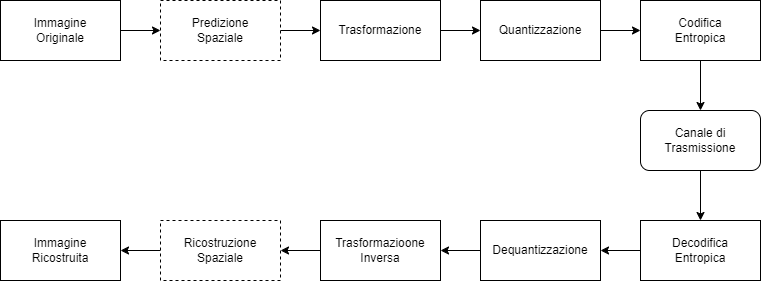
\includegraphics[width=0.8\textwidth]{Immagini/LossyCompressorDiagram.png}
    \caption{Diagramma di compressione Lossy}
    \label{fig:LossyCompressorDiagram}
\end{figure}
